\documentclass[tikz, border = 10pt]{standalone}

%%%<
\usepackage{verbatim}
\usetikzlibrary{calc, intersections}
%%%>

\begin{comment}
:Title: Intersection of the medians of an arbitrary triangle
:Author: Moti Ben-Ari
:Tags: Geometry;Intersections;Median
:Slug: Intersection of medians

TikZ features: name path, name intersections, circle through,
  partway modifier, \foreach, let..in, veclen, \pgfmathparse

  Construction
    Given an arbitrary triangle, its three medians intersect in a
    single point. The intersection divides each median in the
    ratio 2:1.

  Method:
    1. Draw an arbitrary triangle.

    2. Use partway modifiers to locate the midpoint of each
       side and draw the medians.
       
    3. Locate the intersection of two medians and draw a dot.

    4. Locate the intersection of the third median with one of
       the other two to check that it is the same point.

    5. Compute and display the length of each line segment.
       The lengths should be in the ratio 2:1
       (within rounding error).
\end{comment}

\begin{document}

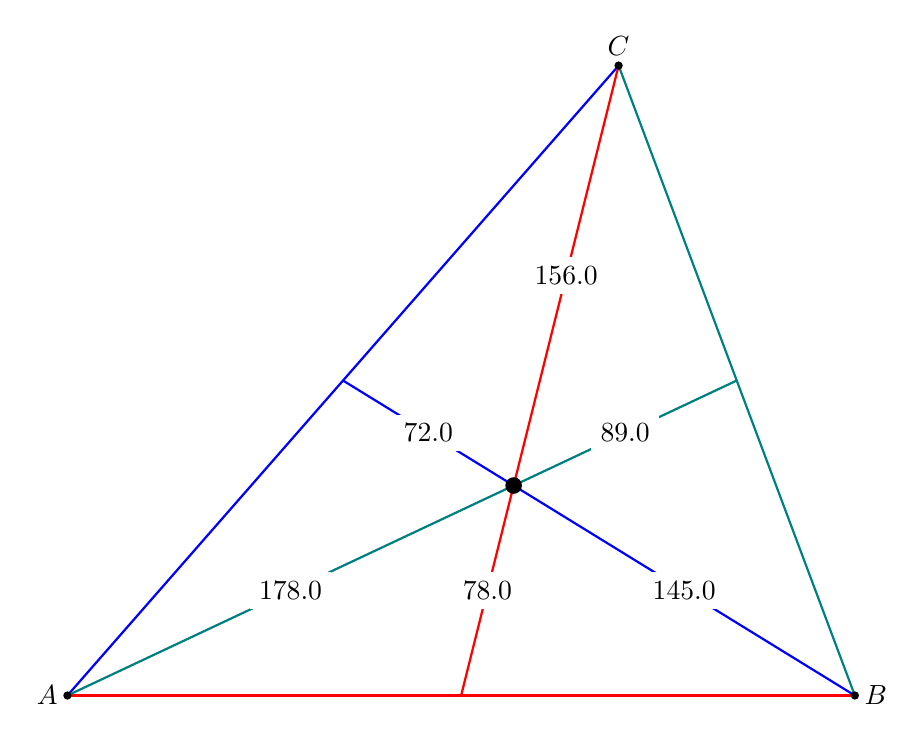
\begin{tikzpicture}
  
  % Define the coordinates of an arbitrary triangle,
  %   label the vertices
  
  \coordinate[label = left:$A$]  (A) at ( 0, 0);
  \coordinate[label = right:$B$] (B) at (10, 0);
  \coordinate[label = above:$C$] (C) at ( 7 ,8);
  
  % Draw the triangle, each side in a different color.
  
  \draw[blue, thick] (A) -- (C);
  \draw[red,  thick] (A) -- (B);
  \draw[teal, thick] (B) -- (C);

  % The coordinates of medians are obtained using partway 
  %   modifier .5 between the vertices of each side.
  
  \coordinate (AB) at ($(A) ! .5 ! (B)$);
  \coordinate (BC) at ($(B) ! .5 ! (C)$);
  \coordinate (AC) at ($(A) ! .5 ! (C)$);
  
  % Draw the medians and name them.

  \draw[teal, thick, name path = Amedian] (A) -- (BC);
  \draw[blue, thick, name path = Bmedian] (B) -- (AC);
  \draw[red,  thick, name path = Cmedian] (C) -- (AB);
  
  % Draw dots at vertices after drawing the lines
  %   so the lines won't cover the vertices

  \fill (A) circle (1.5pt);
  \fill (B) circle (1.5pt);
  \fill (C) circle (1.5pt);
  
  % Get the intersection of two medians and draw a largedot

  \path [name intersections = {% % The comment is necessary!
    of = Amedian and Bmedian,
    by = {intersection}
    }];
  \fill (intersection) circle(2pt);
  
  % Get the intersection with the third median to check
  %   that it is the same point.
  
  \path [name intersections = {% % The comment is necessary!
    of = Amedian and Cmedian,
    by = {intersection2}
    }];
  \fill (intersection2) circle(3pt);

  % If you see two large dots, something is wrong!!!

  % Label each segment
  %   \foreach iterates through the six points:
  %     the vertices of the triangle and the intersections
  %     of the medians with the sides.

  \foreach \point in {A, BC, B, AC, C, AB}
    %
    % Display the label halfway between a point and the
    %   intersection of the medians
    \draw ($(\point) ! .5 ! (intersection)$)
      %
      let
        % ($ (intersection) - (\point) $) is the vector that is
        %   the difference between (intersection) and (\point).
        % \p1 is the coordinate \x1,\y1 of this vector (see below).
        \p1 = ($ (intersection) - (\point) $)
      %
      in
        % veclen(\x1, \y1) is the length \sqrt{\x1^2+\y1^2}.
        % This is rounded to the nearest integer.
        % \pgfmathresult returns the result of the evaluation of
        %   the expression in \pgmathparse.
        % This is used to place a label halfway between
        %   (intersection) and (\point).
      %
      node[fill=white] {\pgfmathparse{
             round(
               veclen(\x1,\y1)
             )
           }
           \pgfmathresult
      };

\end{tikzpicture}

  %  Note:
  %    Section 4.1.3 of the TikZ & PGF Manual is somewhat confusing
  %      in that it talks about the "coordinate" of a vector.
  %    A vector does not have "a" coordinate, but rather the 
  %      two coordinates of its source node and target node, or
  %     the coordinate of its source node
  %     and its direction and length.
  %   \p1 is really the coordinate (\x1,\y1) of the target node
  %      _if_ the source node is translated to (0,0).
  %    That is why the length of the vector is \sqrt{\x1^2+\y1^2}
  %      as written in the manual.
  
  %  Draw the following picture to verify this
  %    (where 0.03528 converts points to centimeters).
  %  Even though the vector goes from (3,3) to (4,4),
  %    \p1 is (1,1) and veclen(\x1,\y1) is \approx \sqrt{2}.
  
  %  \begin{tikzpicture}
  %		\coordinate (A) at (3, 3);
  %		\coordinate (B) at (4, 4);
  %	  \draw (A) -- (B);	
  %	  \draw 
  %	       let
  %	         \p1 = ($ (B) - (A) $)
  %		   in
  %		     node[left]  {\pgfmathparse{\x1*0.03528}\pgfmathresult}
  %		     node[right] {\pgfmathparse{\y1*0.03528}\pgfmathresult}
  %		     node[below,yshift=-8pt]
  %	         {\pgfmathparse{veclen(\x1,\y1)*0.03528}\pgfmathresult};
  %	\end{tikzpicture}

\end{document}
